Для начала мы преобразуем изображение в черно-белое.

\begin{figure}[ht!]
    \centering
    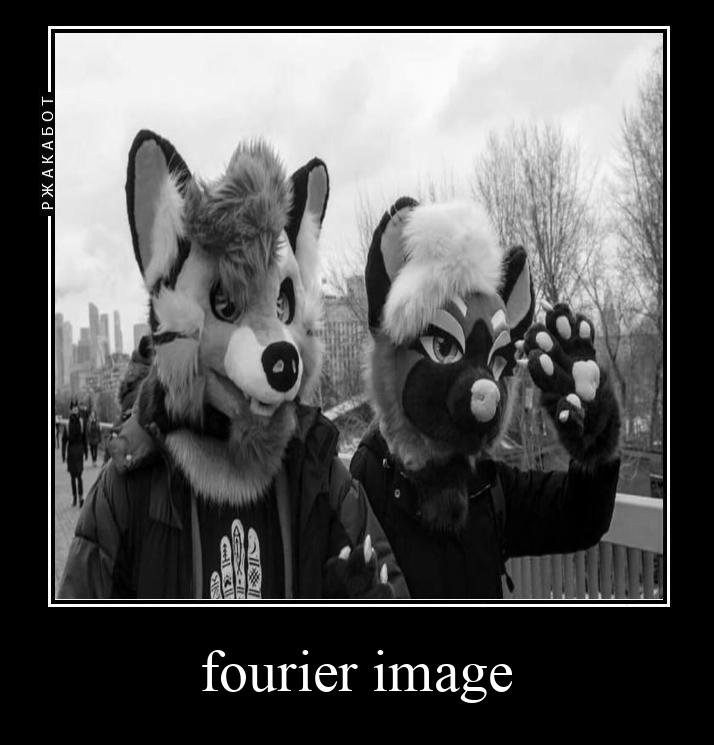
\includegraphics[width=0.5\textwidth]{/Users/nikolajprovorov/Yandex.Disk-368690@edu.itmo.ru.localized/Lab6_Furry_series/bw.png}
    \caption{Черно-белое изображение}
\end{figure}

Для начала выберу 3 нечетных значения $n = 3, 5, 7$

\subsection{Блочное размытие.}

Создадим 3 матрицы ядра блочного размытия. Для этого используем команду 

\begin{equation}
    ones(n)/(n^2)
\end{equation}

\clearpage

Посмотрим на результаты применения ядер к изображению.

\begin{figure}[ht!]
    \centering
    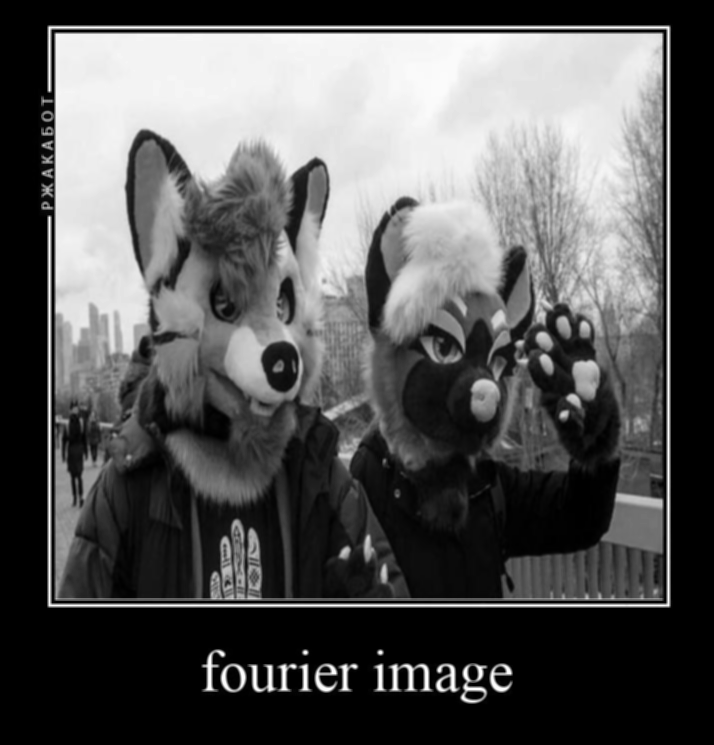
\includegraphics[width=0.5\textwidth]{/Users/nikolajprovorov/Yandex.Disk-368690@edu.itmo.ru.localized/Lab6_Furry_series/block_3.png}
    \caption{Блочное размытие с $n = 3$}
\end{figure}

\begin{figure}[ht!]
    \centering
    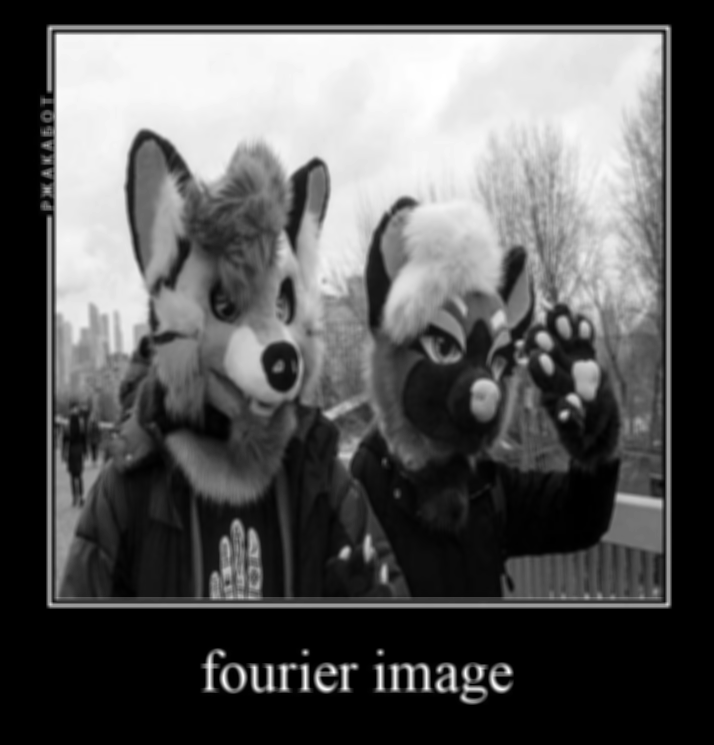
\includegraphics[width=0.5\textwidth]{/Users/nikolajprovorov/Yandex.Disk-368690@edu.itmo.ru.localized/Lab6_Furry_series/block_5.png}
    \caption{Блочное размытие с $n = 5$}
\end{figure}

\clearpage

\begin{figure}[ht!]
    \centering
    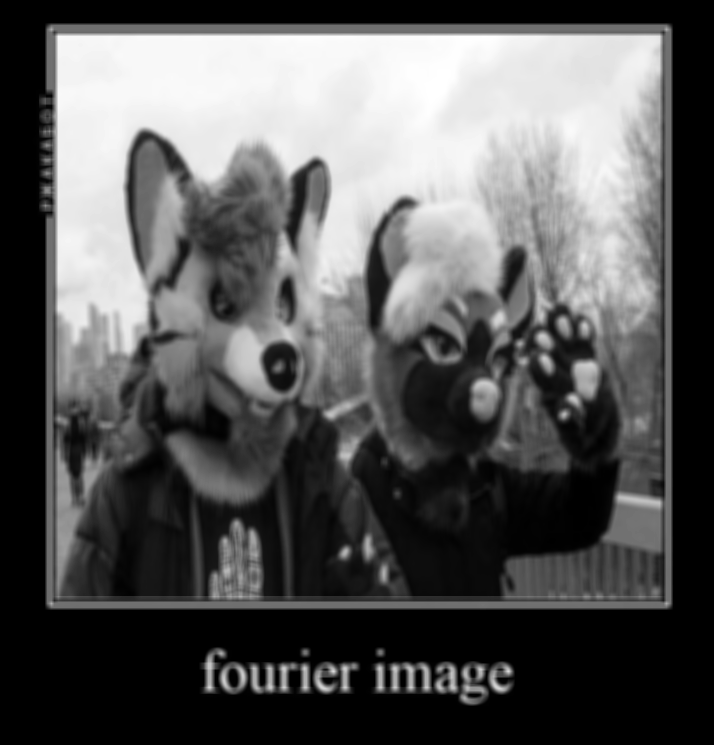
\includegraphics[width=0.5\textwidth]{/Users/nikolajprovorov/Yandex.Disk-368690@edu.itmo.ru.localized/Lab6_Furry_series/block_7.png}
    \caption{Блочное размытие с $n = 7$}
\end{figure}

\subsection{Размытие Гаусса.}

Применим фильтр Гаусса к изображению.

\begin{figure}[ht!]
    \centering
    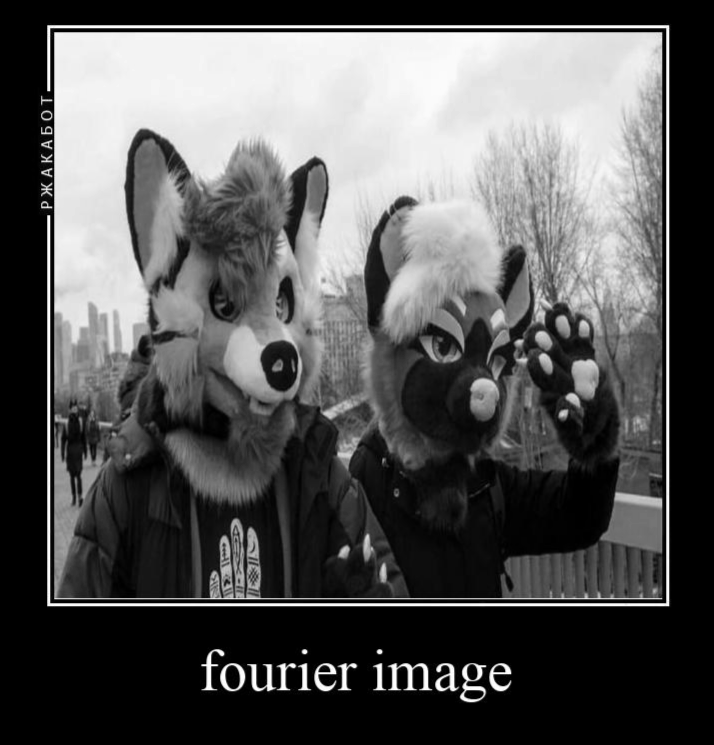
\includegraphics[width=0.5\textwidth]{/Users/nikolajprovorov/Yandex.Disk-368690@edu.itmo.ru.localized/Lab6_Furry_series/gaussian_3.png}
    \caption{размытие Гаусса с $n = 3$}
\end{figure}

\clearpage

\begin{figure}[ht!]
    \centering
    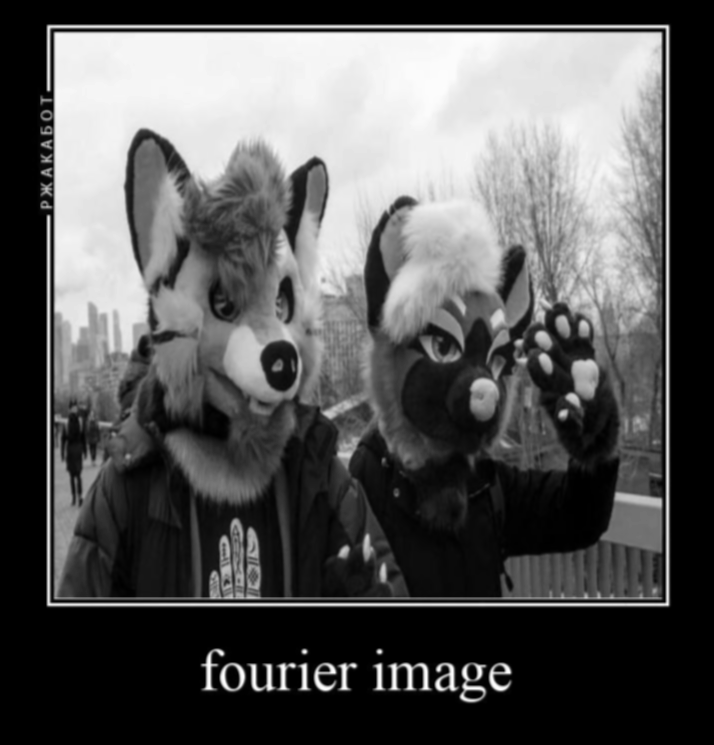
\includegraphics[width=0.5\textwidth]{/Users/nikolajprovorov/Yandex.Disk-368690@edu.itmo.ru.localized/Lab6_Furry_series/gaussian_5.png}
    \caption{размытие Гаусса с $n = 5$}
\end{figure}

\begin{figure}[ht!]
    \centering
    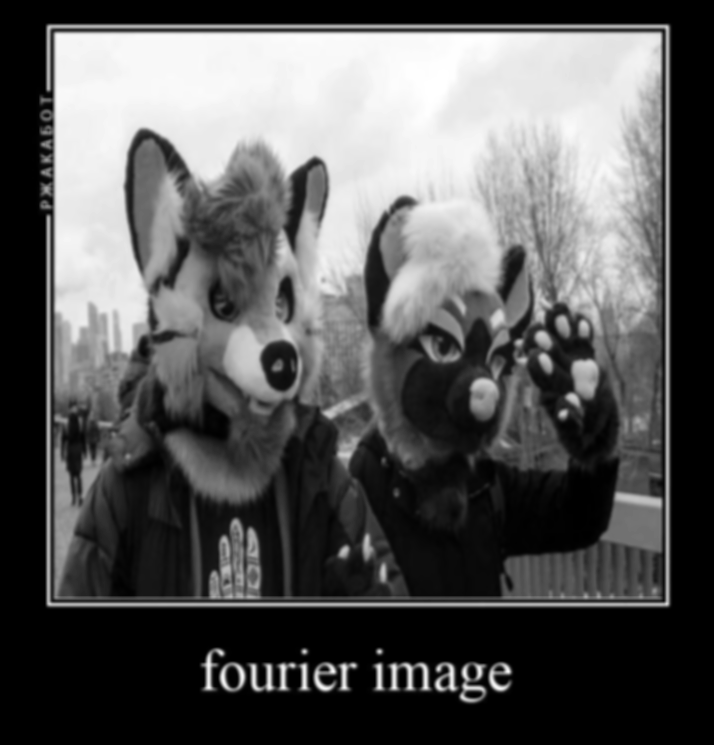
\includegraphics[width=0.5\textwidth]{/Users/nikolajprovorov/Yandex.Disk-368690@edu.itmo.ru.localized/Lab6_Furry_series/gaussian_7.png}
    \caption{размытие Гаусса с $n = 7$}
\end{figure}

\clearpage

Теперь посмотрм что там с фурье-котовасией.

\begin{figure}[ht!]
    \centering
    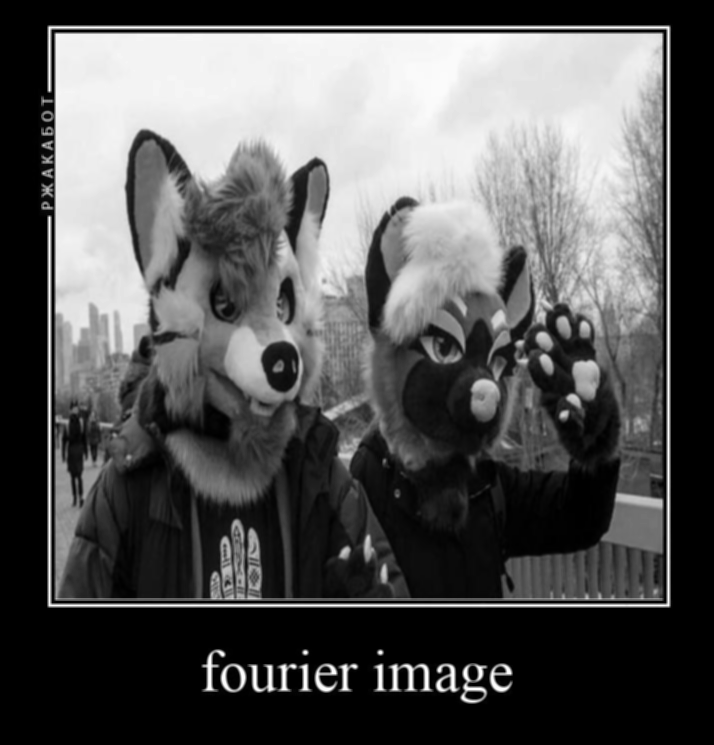
\includegraphics[width=0.5\textwidth]{/Users/nikolajprovorov/Yandex.Disk-368690@edu.itmo.ru.localized/Lab6_Furry_series/block_3.png}
    \caption{Блочное размытие с $n = 3$ (через фурье)}
\end{figure}

\begin{figure}[ht!]
    \centering
    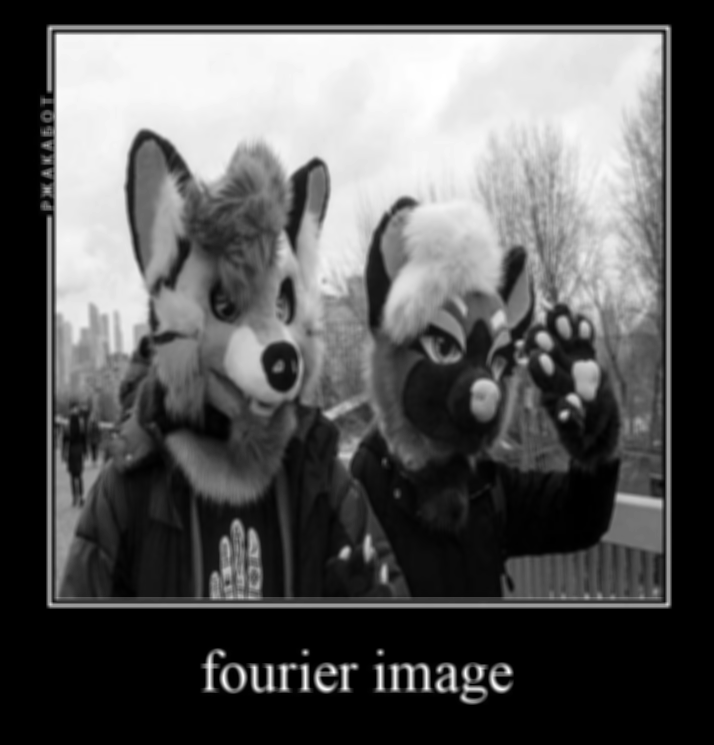
\includegraphics[width=0.5\textwidth]{/Users/nikolajprovorov/Yandex.Disk-368690@edu.itmo.ru.localized/Lab6_Furry_series/block_5.png}
    \caption{Блочное размытие с $n = 5$ (через фурье)}
\end{figure}

\clearpage

\begin{figure}[ht!]
    \centering
    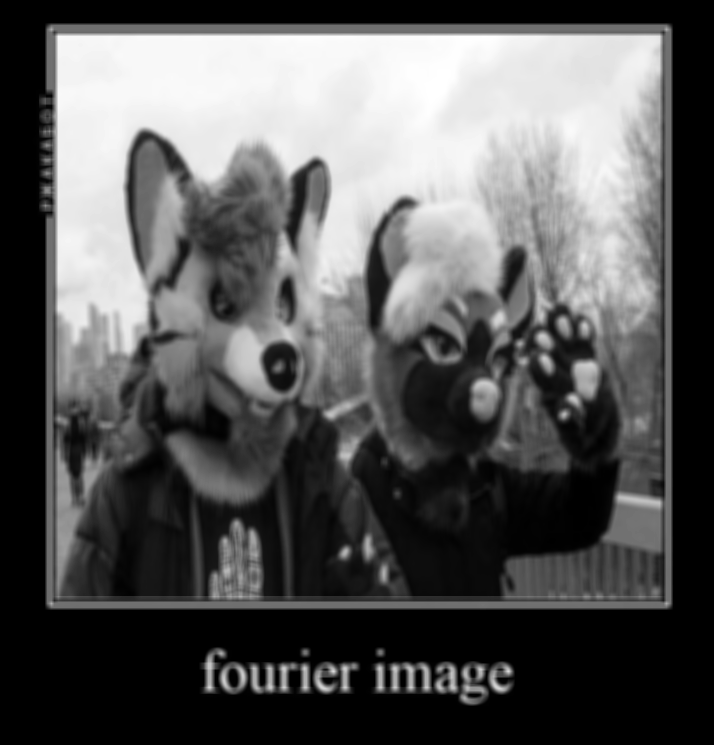
\includegraphics[width=0.5\textwidth]{/Users/nikolajprovorov/Yandex.Disk-368690@edu.itmo.ru.localized/Lab6_Furry_series/block_7.png}
    \caption{Блочное размытие с $n = 7$ (через фурье)}
\end{figure}

\begin{figure}[ht!]
    \centering
    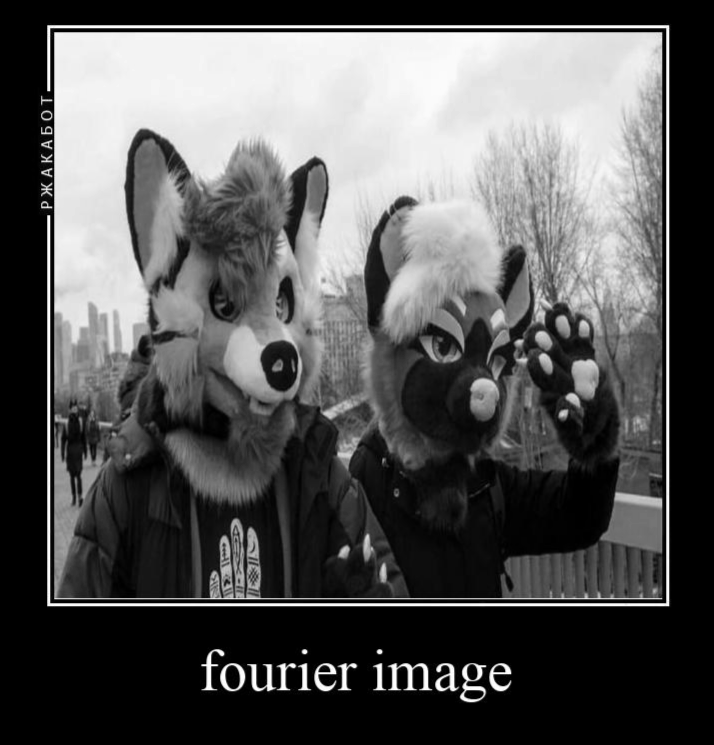
\includegraphics[width=0.5\textwidth]{/Users/nikolajprovorov/Yandex.Disk-368690@edu.itmo.ru.localized/Lab6_Furry_series/gaussian_3.png}
    \caption{размытие Гаусса с $n = 3$ (через фурье)}
\end{figure}

\clearpage

\begin{figure}[ht!]
    \centering
    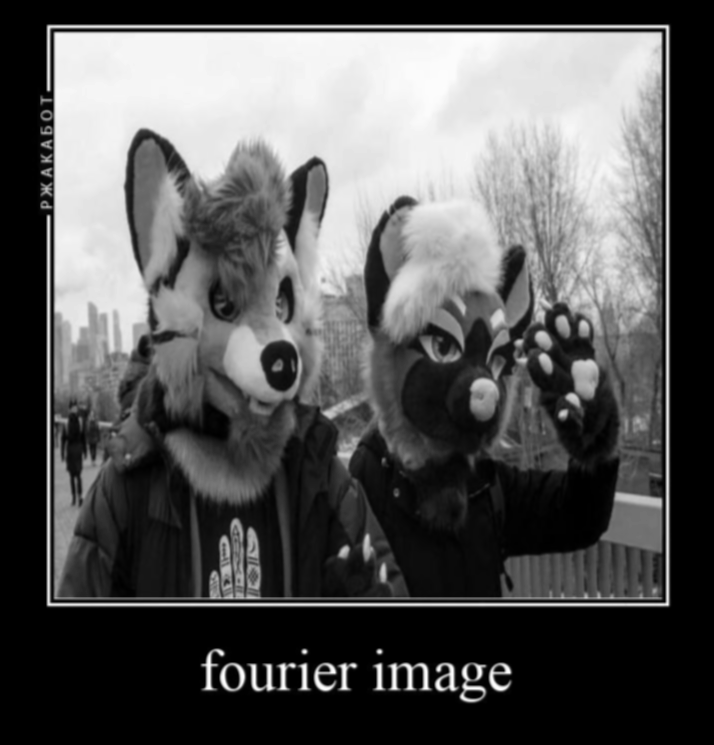
\includegraphics[width=0.5\textwidth]{/Users/nikolajprovorov/Yandex.Disk-368690@edu.itmo.ru.localized/Lab6_Furry_series/gaussian_5.png}
    \caption{размытие Гаусса с $n = 5$ (через фурье)}
\end{figure}

\begin{figure}[ht!]
    \centering
    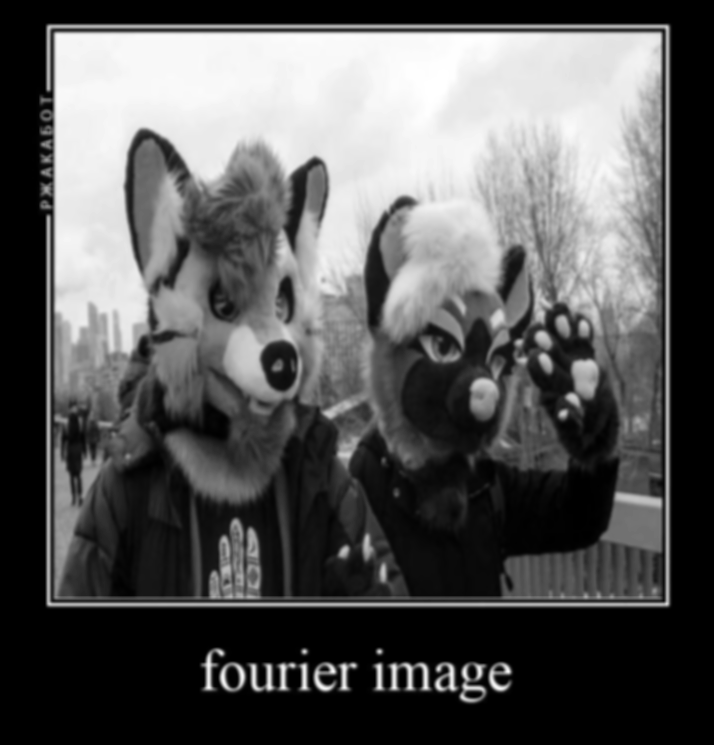
\includegraphics[width=0.5\textwidth]{/Users/nikolajprovorov/Yandex.Disk-368690@edu.itmo.ru.localized/Lab6_Furry_series/gaussian_7.png}
    \caption{размытие Гаусса с $n = 7$ (через фурье)}
\end{figure}

Результаты совпадают, прикольно. Все работает.

Если сравнивать блочное размытие с Гауссом, то можно заметить, что Гауссовское размытие более плавное, чем блочное. Также Гауссовское размытие не так сильно ухудшает качество изображения, как блочное.